\chapter{Конструкторская часть}

    В данном разделе представлены схемы рассматриваемых алгоримтов и их оценка по памяти.
    
    \section{Схемы алгоритмов}
    
        \begin{figure}
            \centering
            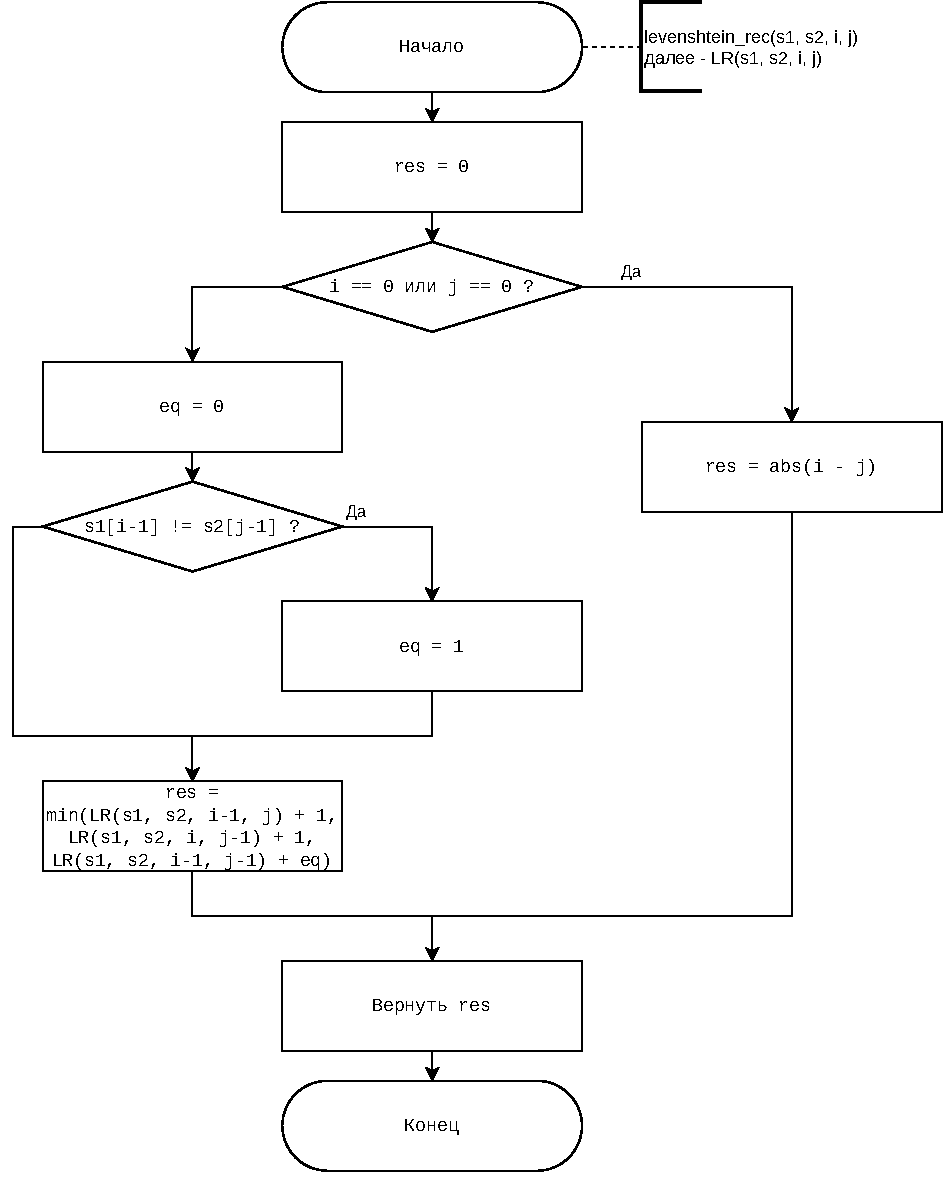
\includegraphics[width=15cm,height=25cm,keepaspectratio]{images/leven_rec.pdf}
            \caption{Рекурсивный алгоритм Левенштейна}
            \label{fig:leven_rec}
        \end{figure}
        
        \begin{figure}
            \centering
            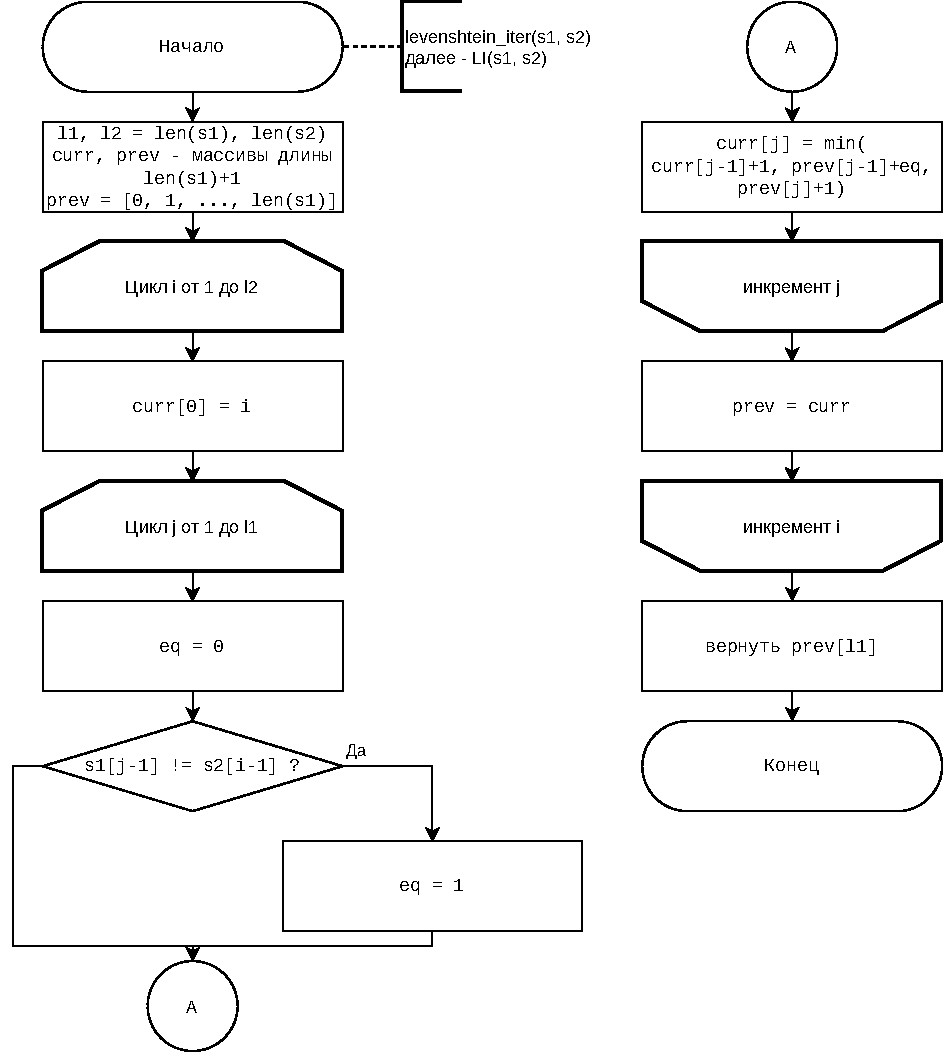
\includegraphics[width=15cm,height=25cm,keepaspectratio]{images/leven_iter.pdf}
            \caption{Рекурсивный алгоритм Левенштейна}
            \label{fig:leven_iter}
        \end{figure}
        
        \begin{figure}
            \centering
            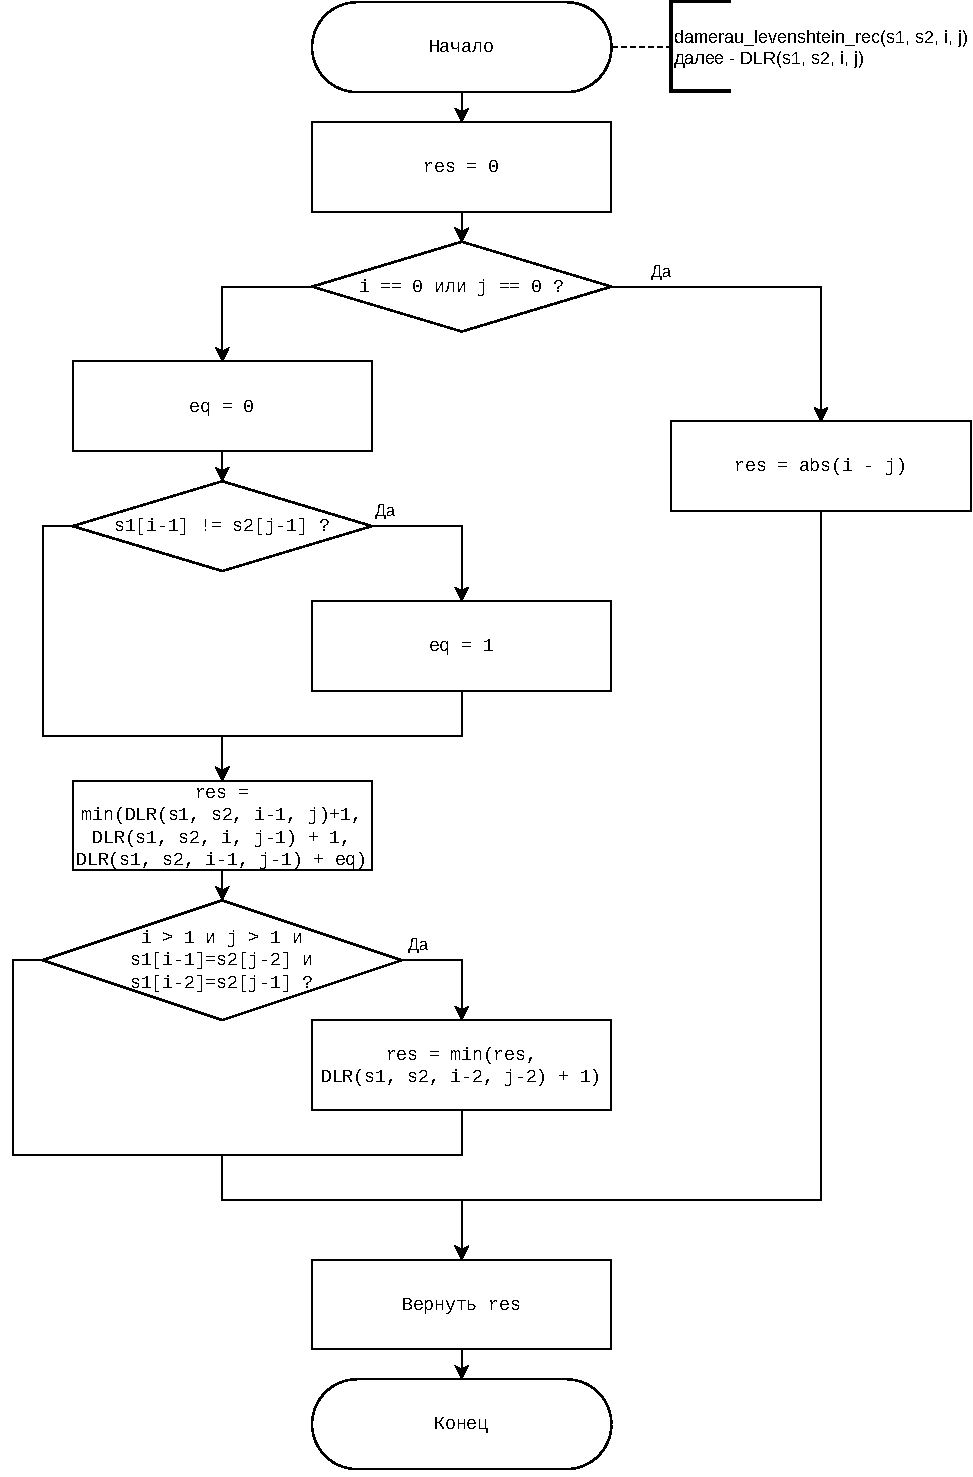
\includegraphics[width=15cm,height=25cm,keepaspectratio]{images/dleven_rec.pdf}
            \caption{Итеративный алгоритм Дамерау - Левенштейна}
            \label{fig:dleven_rec}
        \end{figure}
        
        \begin{figure}
            \centering
            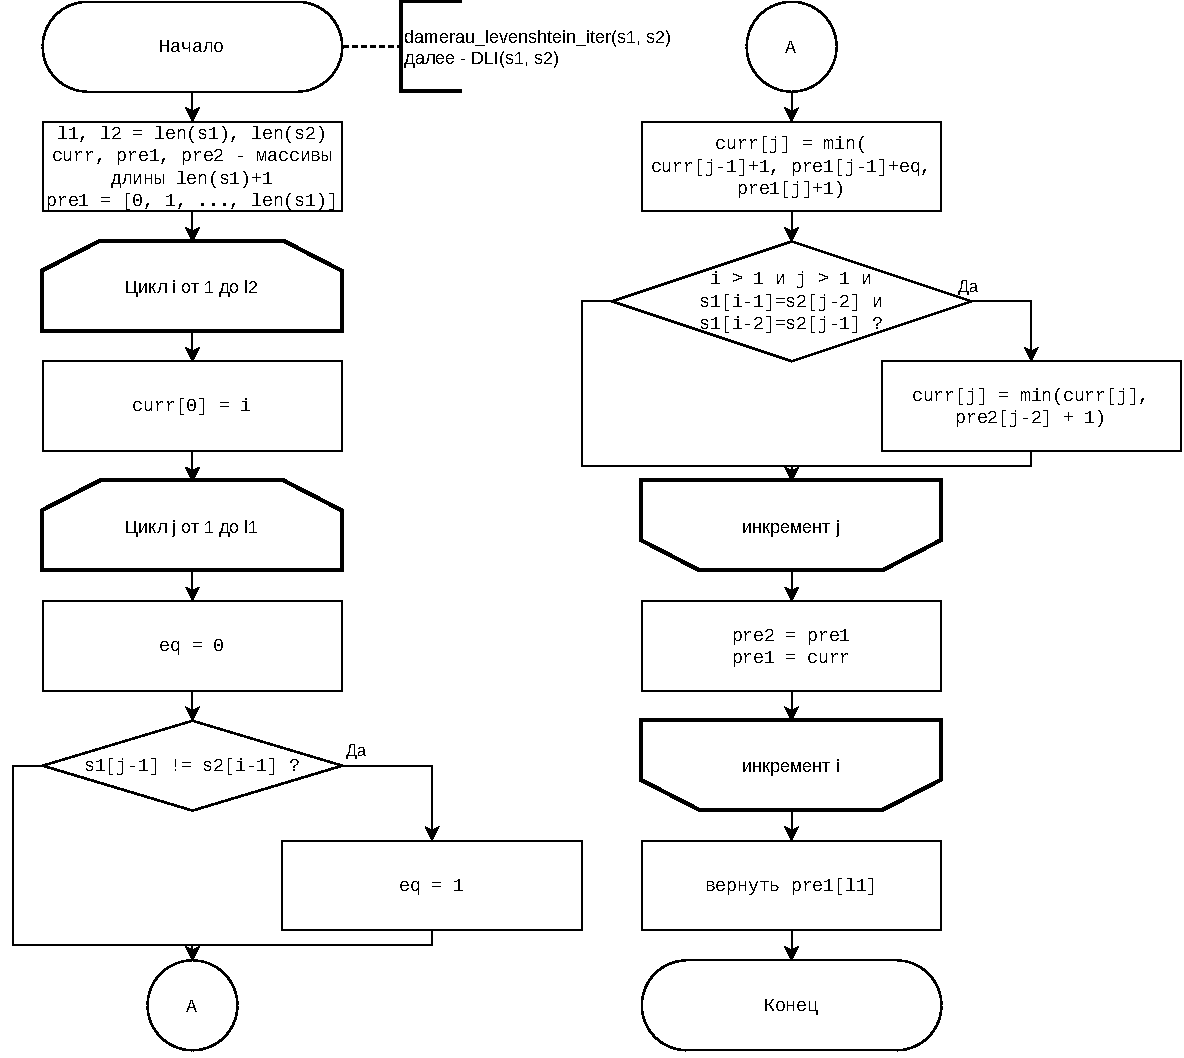
\includegraphics[width=15cm,height=25cm,keepaspectratio]{images/dleven_iter.pdf}
            \caption{Рекурсивный алгоритм Дамерау - Левенштейна}
            \label{fig:dleven_iter}
        \end{figure}
    
    \clearpage
    
    \section{Оценка памяти}
    
        Алгоритмы Левенштейна и Дамерау — Левенштейна не отличаются друг от друга с точки зрения использования памяти, следовательно, достаточно рассмотреть лишь разницу рекурсивной и матричной реализаций этих алгоритмов.
        
        Максимальная глубина стека вызовов при рекурсивной реализации равна сумме длин входящих строк, соответственно, максимальный расход памяти (\ref{for:99})
        \begin{equation}
        (\mathcal{C}(S_1) + \mathcal{C}(S_2)) \cdot (2 \cdot \mathcal{C}\mathrm{(string)} + 3 \cdot \mathcal{C}\mathrm{(int)}),
        \label{for:99}
        \end{equation}
        где $\mathcal{C}$ — оператор вычисления размера, $S_1$, $S_2$ — строки, $\mathrm{int}$ — целочисленный тип, $\mathrm{string}$ — строковый тип.
        
        Использование памяти при итеративной реализации теоретически равно
        \begin{equation}
        (\mathcal{C}(S_1) + 1) \cdot (\mathcal{C}(S_2) + 1) \cdot \mathcal{C}\mathrm{(int)} + 10\cdot \mathcal{C}\mathrm{(int)} + 2 \cdot \mathcal{C}\mathrm{(string)}.
        \end{equation}

    \section{Структуры данных}
    
        В качестве входных данных алгоритмы принимают 2 строки, по которым рассчитывается искомое расстояние. Выходными данными алгоритма является число - найденное расстояние.
        
        В качестве строк для реализации алгоритма выберем нуль-терминировнаныее строки. Никаких других структур данных не потребуется.
        
    \section*{Вывод}
    \addcontentsline{toc}{section}{Вывод}
    
        На основе теоретических данных, полученных из аналитического раздела были построены схемы требуемых алгоритмов.